\section{Reglerentwurf}
Mit Hilfe der Zustandsraumdarstellung kann über die Rückführung des Zustandvektors eine Regelung entworfen werden. Das folgende Blockschaltbild zeigt den Zusammenhang der Systemmatrizen und der Reglermatrix $\textbf{F}$, welche zur Berechnung der Stellgröße $u=T_M$ dient.

\begin{figure}[h]
\label{Regelkreis_pic}
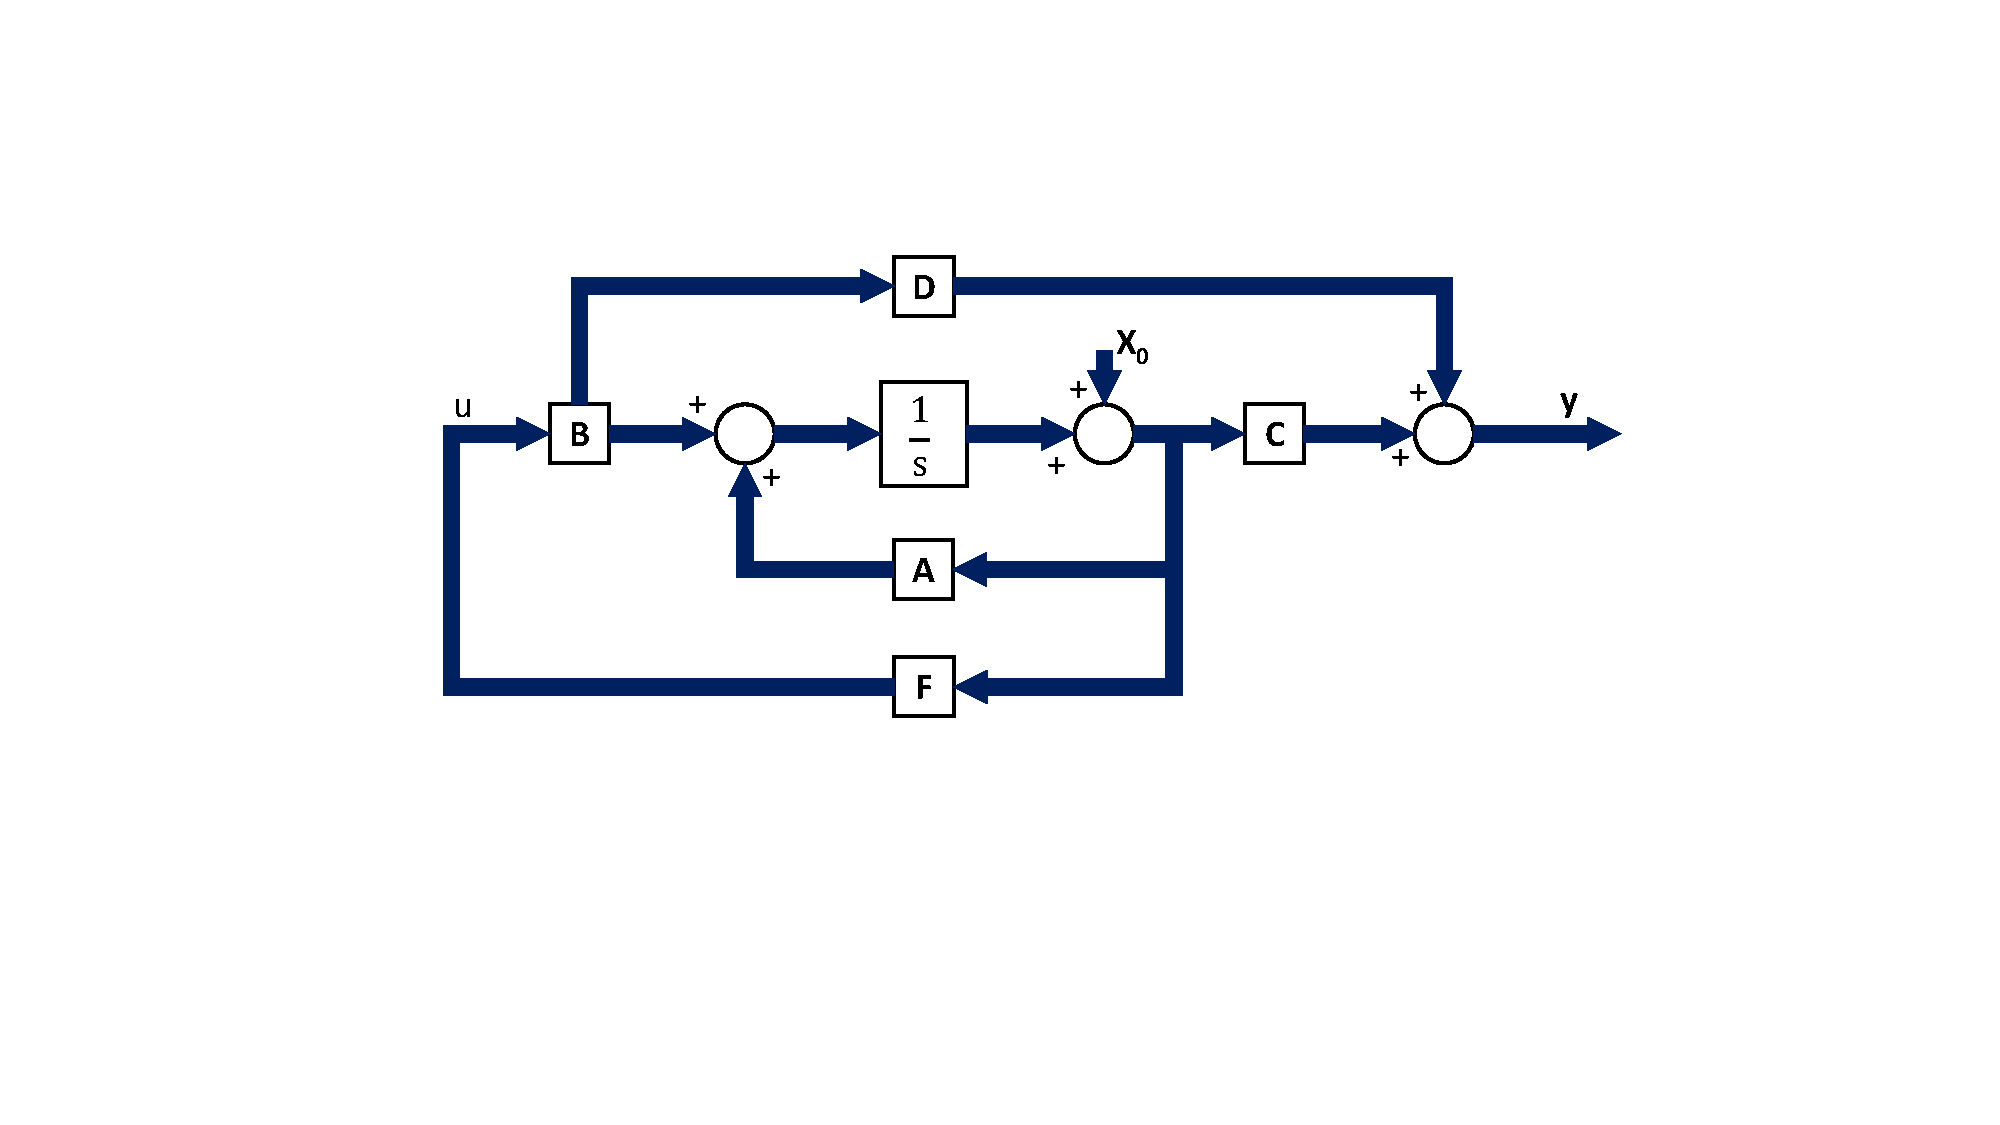
\includegraphics[width=\linewidth, trim={0 6.5cm 0 3.5cm}, clip]{Regelkreis}
\caption{Blockschaltbild Regelkreis, Quelle: eigene Darstellung, Inhalt aus \cite{RT2}}
\end{figure}

Die Stellgröße $u$ wird von einem Mikrokontroller mit einer Abtatsperiod $T_a = 20ms$ berechnet. Folglich handelt es sich um eine digitale Regelung. Um das Verhalten des diskreten Systems zu beschreiben müssen die diskreten Systemmatrizen $\textbf{A}_d$, $\textbf{B}_d$, $\textbf{C}_d$ und $\textbf{D}_d$ berechnet werden. Hierfür gilt nach \cite{RT2}:

\begin{equation}
\textbf{S} = T_a \sum_{v=0}^{\infty} \textbf{A}^v \frac{T^v}{(v+1)!}
\end{equation}
\begin{equation}
\textbf{A}_d = \textbf{I} + \textbf{S} \cdot \textbf{A}
\end{equation}
\begin{equation}
\textbf{B}_d = \textbf{S} \cdot \textbf{B}
\end{equation}
\begin{equation}
\textbf{C}_d = \textbf{C}
\end{equation}
\begin{equation}
\textbf{D}_d = \textbf{D}
\end{equation}

Die Reglermatrix $\textbf{F}$ wird als optimaler Zustandsregler nach dem quadratischen Gütekriterium entworfen. Die diskrete Gütefunktion für dieses System lautet:

\begin{equation}
\label{costfunction_equation}
I = \sum_{k=1}^\infty \textbf{x}^T(k) \cdot \textbf{Q} \cdot \textbf{x}(k) + R\cdot u(k)^2
\end{equation}

Die Matrizen $\textbf{Q}$ und $\textbf{R}$ stellen Gewichtungen der Zustands- und Stellgrößen dar. Die Ausgangswerte dieser Matrizen werden mit der Faustformel nach (\cite{lqrnotes}) berechnet. Ggf. können die Werte anschließend angepasst werden um die Reglergüte weiter zu verbessern.

\begin{equation}
\textbf{Q} = \begin{pmatrix}
\frac{1}{(\varphi_{max})^2} & 0 & 0 \\
0 & \frac{1}{(\dot{\varphi}_{max})^2} & 0 \\
0 & 0 & \frac{1}{(\dot{\psi}_{max})^2} \\
\end{pmatrix}
\end{equation}
\begin{equation}
R = \begin{pmatrix}
\frac{1}{(T_{M,max})^2}
\end{pmatrix}
\end{equation}

Die Reglermatrix $\textbf{F}$ muss die Eigenschaft besitzen die Gütefunktion (\ref{costfunction_equation}) zu minimieren. Dieses Problem wird mit Hilfe von der Matlab-Funktion \textit{lqrd} numerisch gelöst.